%% ma: L11-B01-0011
%% lop: 11
%% chuong: 1
%% bai: 1
%% dang: 11.1.10
%% loai: TN4
%% muc: NB
%% dap_an: "A"
%% nguon: "de-on-tap-giua-ki-1-toan-11-nam-2026-2027-truong-thpt-ngo-quyen-da-nang.pdf (M09, Đề ôn tập giữa kì 1 Toán 11 THPT Ngô Quyền, Đà Nẵng), Mã đề 0113, Phần I Câu 1"
%% kien_thuc: "Bài 1 (giá trị lượng giác của góc lượng giác)"
%% trang_thai: cho-duyet
%% ly_do: "Dạng mới đề xuất 11.1.10"
\begin{ex}
Cho góc hình học $uOv$ có số đo $50^\circ$ (như hình vẽ bên dưới). Xác định số đo của các góc lượng giác $(Ou;Ov)$.
\begin{center}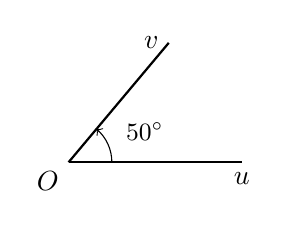
\begin{tikzpicture}[scale=1.1]
\draw[thick] (0,0)--(2,0) node[below] {$u$};
\draw[thick] (0,0)--(50:1.8) node[left] {$v$};
\node[below left] at (0,0) {$O$};
\draw[->] (0.5,0) arc (0:50:0.5);
\node at (22:0.95) {\small$50^\circ$};
\end{tikzpicture}\end{center}
\choice{\True $50^\circ+k360^\circ$ $(k\in\mathbb Z)$}{$-50^\circ+k360^\circ$ $(k\in\mathbb Z)$}{$50^\circ+k180^\circ$ $(k\in\mathbb Z)$}{$-50^\circ+k180^\circ$ $(k\in\mathbb Z)$}
\loigiai{Quay tia $Ou$ ngược chiều kim đồng hồ một góc $50^\circ$ thì đến tia $Ov$; các góc lượng giác $(Ou;Ov)$ có số đo $50^\circ+k360^\circ$ $(k\in\mathbb Z)$.}
\end{ex}
